\section{Alfadian Owen (1174091)}
\subsection{Instalasi Map Server}
\begin{enumerate}
    \item Download aplikasi ms4w melalui website official
    \hfill\break
    \begin{figure}[H]
		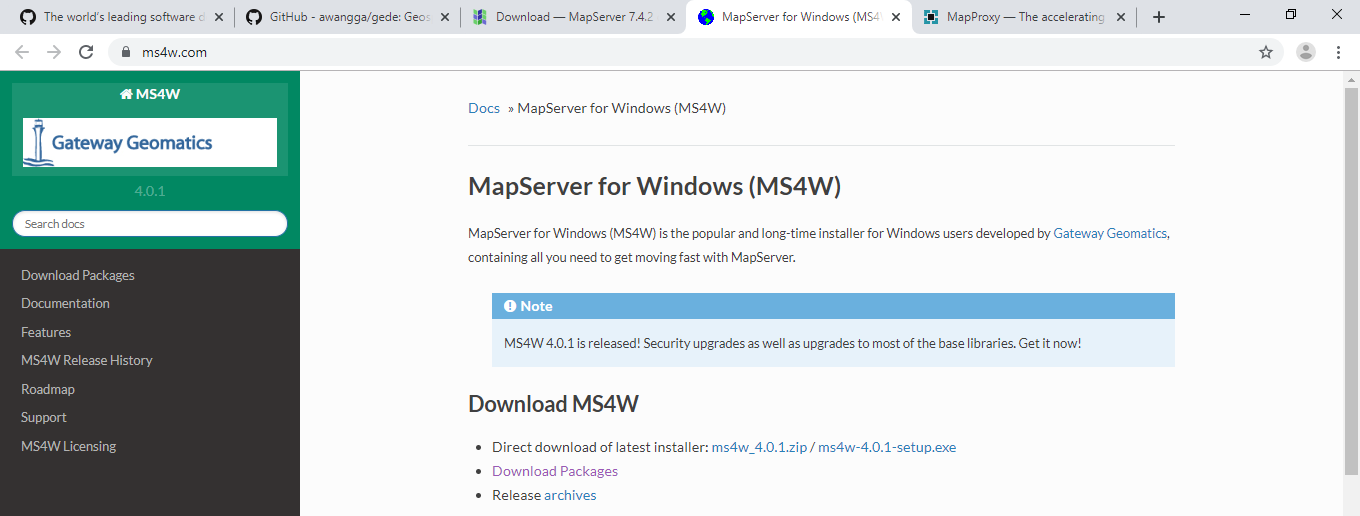
\includegraphics[width=4cm]{figures/tugas4/1174091/1.png}
		\centering
		\caption{Download}
    \end{figure}
    \hfill\break

    \item Pilih Full Install
    \hfill\break
    \begin{figure}[H]
		
\includegraphics[width=4cm]{figures/tugas4/1174091/2.png}
		\centering
		\caption{Download}
    \end{figure}
    \hfill\break

\end{enumerate}

\subsection{Konfigurasi Map Server}
setelah selesai menginstall sekarang konfigurasi file ms4w nya
\begin{enumerate}
  \item Buka Folder ms4w kemudian apache lalu conf
  \hfill\break
    \begin{figure}[H]
		
\includegraphics[width=4cm]{figures/tugas4/1174091/3.png}
		\centering
		\caption{Konfigurasi}
    \end{figure}

  \item Buka file httpd.conf pada line 52 ubah listen 80 menjadi 1000 agar tidak konflik dengan XAMPP.
  \hfill\break
    \begin{figure}[H]
		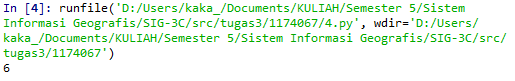
\includegraphics[width=4cm]{figures/tugas4/1174091/4.png}
		\centering
		\caption{Konfigurasi}
    \end{figure}

  \item tekan windows+r dan buka services.msc
  \hfill\break
    \begin{figure}[H]
		
\includegraphics[width=4cm]{figures/tugas4/1174091/5.png}
		\centering
		\caption{Konfigurasi}
    \end{figure}

  \item Klik kanan ApacheMS4WWebServer pilih restart 
  \hfill\break
  \begin{figure}[H]
  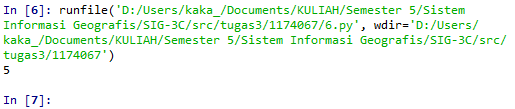
\includegraphics[width=4cm]{figures/tugas4/1174091/6.png}
  \centering
  \caption{Konfigurasi}
  \end{figure}

\end{enumerate}



\subsection{Instalasi MapProxy}
\begin{enumerate}
  \item Buka CMD
  \item ketik pip install MapProxy
  \hfill\break
  \begin{figure}[H]
  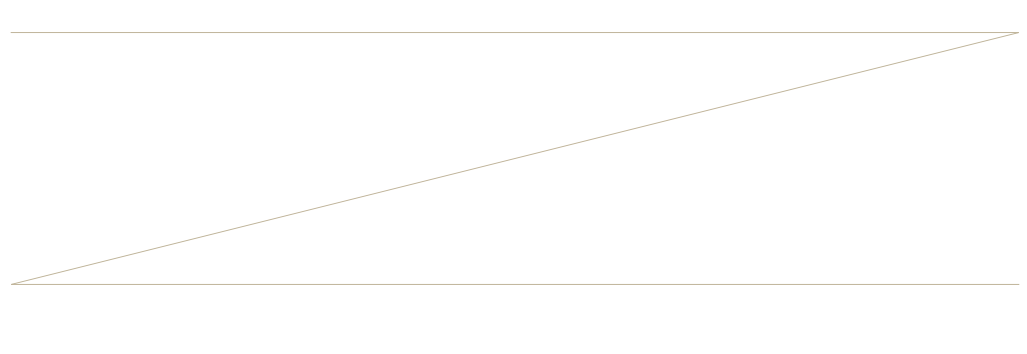
\includegraphics[width=4cm]{figures/tugas4/1174091/7.png}
  \centering
  \caption{Instalasi}
  \end{figure}
\end{enumerate}

\subsection{Membuka map menggunakan MapProxy}
\begin{enumerate}
  \item clone git dari https://github.com/awangga/gede
  \item Buat folder bernama tmp di gede-master
  \hfill\break
  \begin{figure}[H]
  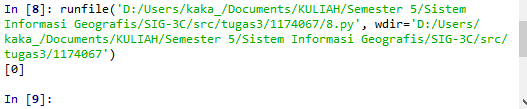
\includegraphics[width=4cm]{figures/tugas4/1174091/8.png}
  \centering
  \caption{Buat folder}
  \end{figure}

  \item buka folder mapproxy lalu edit file agm.yaml
  \hfill\break
  \begin{figure}[H]
  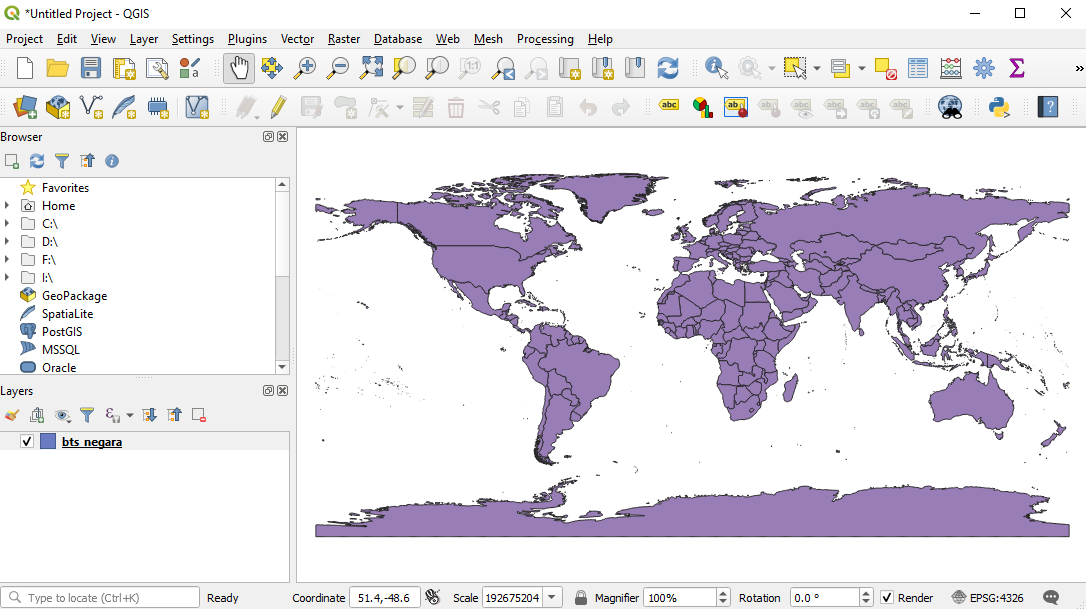
\includegraphics[width=4cm]{figures/tugas4/1174091/9.png}
  \centering
  \caption{File}
  \end{figure}

  \item Pada line 54, masukkan path mapfile yang ada pada folder gede yang telah anda clone pada binary masukkan path mapserv.exe yang telah anda install
  \hfill\break
  \begin{figure}[H]
  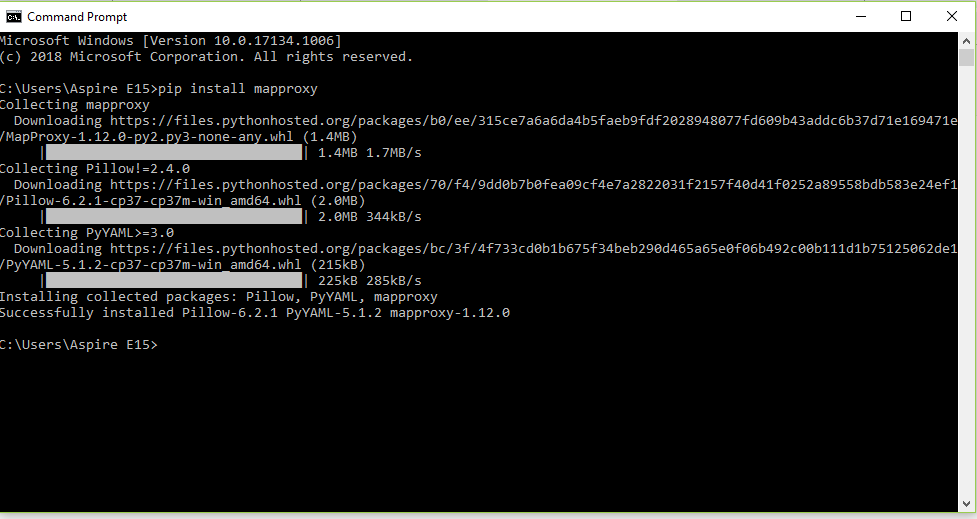
\includegraphics[width=4cm]{figures/tugas4/1174091/10.png}
  \centering
  \caption{Edit amg.yaml}
  \end{figure}




  \item buka aplikasi MS4W-Shell
  

  \item buka lokasi folder gede kita yang tadi telah di clone
  

  \item buka folder mapproxy yang ada pada folder gede


  \item ketikkan "mapproxy-util serve-develop ./agm.yaml" untuk membuka aplikasi mapproxy
  \hfill\break
  \begin{figure}[H]
  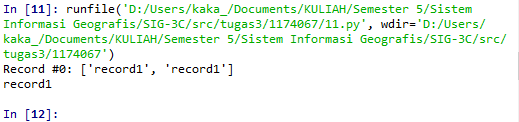
\includegraphics[width=4cm]{figures/tugas4/1174091/11.png}
  \centering
  \caption{Buka aplikasi mapproxy}
  \end{figure}
  
  \item Buka browser lalu ketikkan 127.0.0.1:8080


  \item lalu klik demo untuk melihat map
  \item lalu klik png pada agm, maka mapproxy akan menampilkan map


\end{enumerate}




